\documentclass[10pt, aspectratio=169]{beamer}
\usepackage{tikz}
\usepackage{xcolor}
\usepackage{graphicx}
\usepackage{amsmath}
\usepackage{listings}
\usepackage{color}
\usepackage{url}
\usepackage{hyperref}
\usepackage{cite}
\usepackage[utf8]{inputenc}
\usepackage{courier}
\usepackage{tabularx} % For adjustable width tables
\usepackage{booktabs} % For better table formatting
\usepackage{array}    % For additional column formatting
\usepackage{ragged2e} % For better text justification
\usepackage{float} % Add to preamble


\lstset{
  basicstyle=\ttfamily\footnotesize,
  keywordstyle=\color{blue},
  commentstyle=\color{gray},
  stringstyle=\color{red},
  showstringspaces=false,
  breaklines=true,
  backgroundcolor=\color{black!5},
  captionpos=b
}

\usetikzlibrary{arrows.meta, positioning, shapes.geometric}


\usetheme{CambridgeUS}
\usecolortheme{dolphin}
\usefonttheme{serif}
\usepackage{fontawesome5}


\title[GEM5 Extensions]{\textbf{GEM5 Extensions}: Broadening Support to Microcontrollers with GUI}
\author{Ashutosh Vishwakarma}
\institute{IIT Jammu}
\date{\today}

\begin{document}

\begin{frame}
  \begin{figure}
    \centering
    \includegraphics[width=0.10\textwidth]{images/iitjammu.png}
    \hspace{1.5cm}
    \includegraphics[width=0.08\textwidth]{images/gem5.png}
    \titlepage
    \centering
    Guide: Dr. Subhasis Bhattacharjee
  \end{figure}
\end{frame}


\begin{frame}{Overview}
  \tableofcontents
\end{frame}

\section{Introduction}
\begin{frame}{What is GEM5?}
  \begin{itemize}
    \item \textbf{GEM5} is a modular platform for computer-system architecture research.
    \item It merges features from \textbf{M5} (full system simulator) and the original \textbf{GEM5} (CPU modeling framework).
    \item Supports simulation of a wide range of ISAs: \textbf{x86, ARM, RISC-V, SPARC, MIPS}, and more.
    \item Enables both \textbf{system-level} and \textbf{cycle-accurate} CPU simulation.
    \item Widely used for:
      \begin{itemize}
        \item Academic and industrial architecture research
        \item Performance analysis and profiling
        \item Design-space exploration
      \end{itemize}
    \item \textbf{Open-source} and highly extensible — ideal for custom architecture extensions.
  \end{itemize}
\end{frame}


\begin{frame}{What is GEM5?}
  \begin{itemize}
    \item \textbf{GEM5} is structured into multiple components that interact modularly:
    \begin{itemize}
      \item \textbf{CPU Models}: TimingSimple, Minor, O3, and atomic models.
      \item \textbf{Memory System}: Includes caches, memory controllers, and interconnects.
      \item \textbf{Devices}: Peripheral models like UART, timers, and disk controllers.
      \item \textbf{ISAs}: Support for multiple instruction sets like ARM, RISC-V, x86, etc.
      \item \textbf{Full System vs. Syscall Emulation Modes}
    \end{itemize}
    \item Designed to be \textbf{modular and extensible}, allowing researchers to plug in new components.
  \end{itemize}
\end{frame}

\begin{frame}{What is GEM5?}
  \begin{itemize}
    \item \textbf{Hybrid C++ and Python Design}:
    \begin{itemize}
      \item Core simulation engine written in C++ for performance.
      \item Configuration and modeling interfaces written in Python for flexibility.
    \end{itemize}

    \item \textbf{User Interaction}:
    \begin{itemize}
      \item Users write Python scripts to define system architecture, CPUs, memory, peripherals.
      \item These scripts internally call C++ classes and methods via Python bindings.
    \end{itemize}

    \item \textbf{Simulation Flow}:
    \begin{itemize}
      \item Python config → System Instantiation → Simulation via C++ backend.
    \end{itemize}
  \end{itemize}
\end{frame}

\begin{frame}{What is GEM5?}
  \centering
    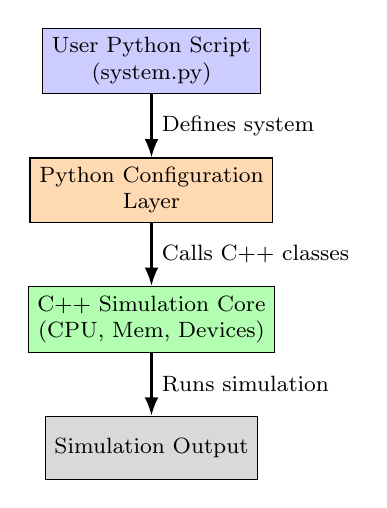
\begin{tikzpicture}[
    node distance=0.8cm and 1.5cm,
    every node/.style={font=\footnotesize},
    box/.style={rectangle, draw, minimum width=2.5cm, minimum height=0.8cm, align=center},
    arrow/.style={-{Latex}, thick}
  ]
    \node[box, fill=blue!20] (user) {User Python Script\\(system.py)};
    \node[box, fill=orange!30, below=of user] (pycfg) {Python Configuration\\Layer};
    \node[box, fill=green!30, below=of pycfg] (cppcore) {C++ Simulation Core\\(CPU, Mem, Devices)};
    \node[box, fill=gray!30, below=of cppcore] (output) {Simulation Output};

    \draw[arrow] (user) -- (pycfg) node[midway, right] {Defines system};
    \draw[arrow] (pycfg) -- (cppcore) node[midway, right] {Calls C++ classes};
    \draw[arrow] (cppcore) -- (output) node[midway, right] {Runs simulation};
  \end{tikzpicture}\\
  \textbf{Figure 1: }Simulation flow in GEM5
\end{frame}


\section{Objectives}
\begin{frame}{Goals}
  \begin{itemize}
    \item Extend support for diverse microcontroller architectures.
    \item Target ISAs include ARM Cortex-M and AVR.
    \item Enable modeling of custom peripherals and I/O devices.
    \item Incorporate interrupt-driven architecture support.
    \item Facilitate real-time performance analysis and monitoring.
    \item Provide tools for debugging and execution trace visualization.
  \end{itemize}
\end{frame}

\begin{frame}{System Overview}
  \centering
  \begin{figure}
    \includegraphics[width=1.0\textwidth]{images/proposed_system.png}
  \end{figure}
  \textbf{Figure 2: }Proposed System Architecture
\end{frame}

\begin{frame}{Why It Matters}
  \begin{itemize}
    \item \textbf{Microcontrollers power the embedded world} — from smart homes to medical devices.
    \item Existing GEM5 support focuses mainly on general-purpose computing architectures.
    \item Extending GEM5 enables researchers to:
    \begin{itemize}
      \item Model real-world embedded and IoT systems.
      \item Explore architectural trade-offs in low-power environments.
      \item Test RTOS behavior and peripheral interactions in a controlled simulation.
    \end{itemize}
    \item Opens doors for hardware-software co-design in constrained systems.
    \item Facilitates early-stage development and validation of next-gen embedded solutions.
  \end{itemize}
\end{frame}

\begin{frame}{Why It Matters}
  \begin{itemize}
    \item \textbf{Existing Simulators:}
    \begin{itemize}
      \item \textit{AVR Simulator, SimAVR, Proteus:} Limited scope, vendor-specific.
      \item \textit{QEMU:} General-purpose, lacks fine-grained modeling for peripherals and interrupts in microcontrollers.
      \item \textit{Renode:} Powerful, but more focused on specific embedded use cases.
    \end{itemize}
    \item \textbf{Limitations:}
    \begin{itemize}
      \item Minimal hardware-software co-design flexibility.
      \item Limited extensibility for new ISAs and custom architectures.
      \item Often lack integrated performance profiling and debugging tools.
    \end{itemize}
    \item \textbf{GEM5-based Simulator:}
    \begin{itemize}
      \item Fully extensible with support for custom ISAs like AVR and ARM Cortex-M.
      \item Integration with real-time operating systems and custom peripherals.
      \item High-level UI for configuring and analyzing simulations.
      \item Enables in-depth architectural research and exploration.
    \end{itemize}
  \end{itemize}
\end{frame}



\section{Approach}
\begin{frame}{Approach}
  \begin{itemize}
    \item \textbf{Step 1: Research and Analysis} – Study GEM5 internals, identify extensible components.
    \item \textbf{Step 2: ISA Integration} – Add support for AVR architecture.
    \item \textbf{Step 3: Peripheral \& Interrupt Modeling} – Develop modules for custom I/O and interrupt logic.
    \item \textbf{Step 4: UI Development} – Build an intuitive visual interface for simulation configuration.
    \item \textbf{Step 5: Debug Tools \& Testing} – Add real-time performance monitoring, debugging, and trace tools.
  \end{itemize}
\end{frame}


\section{Implementation}
\begin{frame}{Step 1: Research and Analysis}
  \begin{itemize}
    \item \textbf{Exploring GEM5 Internals:} 
      \begin{itemize}
        \item Investigated the core components of GEM5 including CPU models, memory systems, and simulation flow.
        \item Found limited developer documentation — referred to the official \href{https://doxygen.gem5.org/develop/index.html}{Doxygen documentation \faLink}.
        \item Studied through 3,358 source files comprising 965,657 lines of code.
      \end{itemize}

    \item \textbf{Studying AVR Architecture:}
      \begin{itemize}
        \item Reviewed instruction set, register architecture, and interrupt handling for AVR microcontrollers.
      \end{itemize}

    \item \textbf{Feasibility Analysis:}
      \begin{itemize}
        \item Evaluated how a lightweight 16-bit AVR ISA could be integrated into GEM5’s CPU model framework.
        \item Focused on maintaining modularity and clean abstraction layers.
      \end{itemize}

    \item \textbf{Initial Outcomes:}
      \begin{itemize}
        \item Conducted a simulation-based evaluation titled \href{https://drive.google.com/file/d/13ZroHuWGLApYXLkeWA3SBIlMh6KzfCqq/view?usp=sharing}{\texttt{Comparative Study on Execution Speed \& CMR of Various ISAs \faLink.}} 
      \end{itemize}
  \end{itemize}
\end{frame}


\begin{frame}{Step 2: ISA Integration}
  \centering
  \includegraphics[width=0.55\textwidth]{images/impl.png}\\
  \textbf{Figure 3: }Dependence of gem5 components on ISA
\end{frame}

\begin{frame}{Step 2: ISA Integration}
  \begin{itemize}
    \item For the project we need to implement:
    \begin{itemize}
      \item ISA Description
      \item Decoder
      \item Fault Interrupts
      \item Predecoder
      \item Python Bindings to CPU \& I/O models.
      \item GUI for the simulator
    \end{itemize}
    \item For the begging a set of basic instructions are being implemented:
    \begin{itemize}
      \item \textbf{Arithmetic Instructions:} ADD, SUB
    \end{itemize}
    \item Current implementation includes:
    \begin{itemize}
      \item ISA Description with two above-mentioned instructions
      \item \texttt{AVRFault} for fault handling
      \item \textbf{Registers:} 32 general-purpose registers (R0-R31), SREG (Status Register)
      \item \textbf{Program Counter (PC):} 16-bit PC for instruction addressing
      \item \textbf{Instruction Fetch and Decode:} Basic fetch-decode-execute cycle
    \end{itemize}
  \end{itemize}
\end{frame}

\begin{frame}[fragile]{Step 2: ISA Integration}
  \begin{figure}
    \centering
      \includegraphics[width=0.8\textwidth]{images/flow.png}\\
      \textbf{Figure 4:} ISA description flow
  \end{figure}
\end{frame}

\begin{frame}[fragile]{Step 2: ISA Integration}
    Traversing the pipeline with `\texttt{add}' instruction:
    \begin{itemize}
      \item Bitfield definition for the instructions to be later used in the decoder: 
      \begin{lstlisting}[language=C++]
        def bitfield OPCODE    <15:10>;
        def bitfield REG_D     <8:4>;
        def bitfield REG_R     <3:0>;
        def bitfield IMM8      <7:0>;
      \end{lstlisting}
    \end{itemize}
\end{frame}

\begin{frame}[fragile]{Step 2: ISA Integration}
  \begin{itemize}
    \item Format declaration for \texttt{add} instruction. The declaration defines the output blocks for the code to be generated:
    \begin{lstlisting}[language=C++]
      def format Add(code, *opt_args) {{
        iop = InstObjParams(name, Name, 'AddOp',
                          {'code': code,
                            'predicate_test': predicateTest,
                            'op_class': 'gem5::enums::IntAlu'
                          },
                          opt_args)
        header_output = AddDeclare.subst(iop)
        decoder_output = AddConstructor.subst(iop)
        decode_block = AddDecode.subst(iop)
        exec_output = AddExecute.subst(iop)
        disasm_output = AddDisassembly.subst(iop)
    }};
    \end{lstlisting}
  \end{itemize}
\end{frame}

\begin{frame}[fragile]{Step 2: ISA Integration}
  \begin{itemize}
    \item Add class declaration including the constructor, execute method, disassembly method and PC advancement method:
    \begin{lstlisting}[language=C++]
      def template AddDeclare {{
        class %(class_name)s : public gem5::AVRISAInst::AVRStaticInst
        {
          public:
            %(class_name)s(gem5::AVRISAInst::MachInst machInst);
            Fault execute(ExecContext *, trace::InstRecord *) const override;
            std::string generateDisassembly(Addr pc,
                const loader::SymbolTable *symtab) const override;
            void advancePC(PCStateBase &pc_state) const;
        };
      }};
    \end{lstlisting}
  \end{itemize}
\end{frame}

\begin{frame}[fragile]{Step 2: ISA Integration}
  \begin{itemize}
    \item Generated C++ code for the Add class from the DSL code above:
    \begin{lstlisting}[language=C++]
      #undef OPCODE
      #define OPCODE	bits(machInst, 15, 10)
      #undef REG_D
      #define REG_D	bits(machInst,  8,  4)
      #undef REG_R
      #define REG_R	bits(machInst,  3,  0)
      #undef IMM8
      #define IMM8	bits(machInst,  7,  0)
      class Add : public gem5::AVRISAInst::AVRStaticInst
      {
        public:
          Add(gem5::AVRISAInst::MachInst machInst);
          Fault execute(ExecContext *, trace::InstRecord *) const override;
          std::string generateDisassembly(Addr pc,
              const loader::SymbolTable *symtab) const override;
          void advancePC(PCStateBase &pc_state) const;
      };
    \end{lstlisting}
  \end{itemize}
\end{frame}


\begin{frame}{Step 2: ISA Integration}
  \begin{itemize}
    \item Getting integration success with these two instructions opened door for further extending the instruction set.
    \item The groundwork for extension is laid out with the fault handling, PC management and register modeling. 
  \end{itemize}
\end{frame}

\section{Future Work}
\begin{frame}{Future Work}
    \begin{itemize}
      \item Develop \texttt{Python} binding for \textbf{AVR CPU} model to execute the AVR instructions.
      \item Implement the memory model the CPU (Harvard architecture although GEM5 currently only supports Von Neumann architecture).
      \item Implement the \texttt{AVRIO} model to handle the I/O operations.
      \item Benchmark testing.
      \item Extracting the runtime statistics from the simulator to a GUI.
    \end{itemize}
  \end{frame}
  

\section{Conclusion}
  \begin{frame}{Conclusion}
  \begin{itemize}
      \item Extended \textbf{GEM5} to support \textbf{microcontroller architectures}, specifically \textbf{AVR}.
      \item Built a foundation for \textbf{custom ISA integration}:
      \begin{itemize}
          \item Instruction decoding
          \item Fault handling
          \item Register modeling
      \end{itemize}
      \item Implemented groundwork for \textbf{interrupt-driven simulation}.
      \item Proposed a plan for \textbf{GUI-based configuration and visualization}.
      \item Enables:
      \begin{itemize}
          \item \textbf{In-depth architectural research}
          \item \textbf{Hardware-software co-design}
          \item \textbf{Early validation} of embedded systems
      \end{itemize}
  \end{itemize}
\end{frame}


\section{References}
\begin{frame}[allowframebreaks]{References}
  \begin{itemize}
    \item[{\bf [1]}] A. Butko, R. Garibotti, L. Ost, and G. Sassatelli, \textbf{\textit{“Accuracy evaluation of GEM5 simulator system,”}} in 7th International Workshop on Reconfigurable and Communication-Centric Systems-on-Chip (ReCoSoC), 2012.
    
    \item[{\bf [2]}] S. V. Bharadwaj and C. K. Vudadha, \textbf{\textit{“Evaluation of x86 and ARM architectures using compute-intensive workloads,”}} in 2022 IEEE International Symposium on Smart Electronic Systems (iSES), 2022.
    
    \item[{\bf [3]}] R. Saha, Y. P. Pundir, S. Yadav, and P. K. Pal, \textbf{\textit{“Impact of size, latency of cache-L1 and workload over system performance,”}} in 2020 International Conference on Advances in Computing, Communication Materials (ICACCM), 2020.
    
    \item[{\bf [4]}] A. D. George, \textbf{\textit{“An overview of RISC vs. CISC,”}} in Proceedings of the Twenty-Second Southeastern Symposium on System Theory, 1990.
    
    \item[{\bf [5]}] M. Ling, X. Xu, Y. Gu, and Z. Pan, \textbf{\textit{“Does the ISA really matter? A simulation-based investigation,”}} in 2019 IEEE Pacific Rim Conference on Communications, Computers and Signal Processing (PACRIM), 2019.
    
    \item[{\bf [6]}] T. Jamil, \textbf{\textit{“RISC versus CISC,”}} IEEE Potentials, vol. 14, no. 3, pp. 13–16, 1995.
    
    \item[{\bf [7]}] A. A. Abudaqa, T. M. Al-Kharoubi, M. F. Mudawar, and A. Kobilica, \textbf{\textit{“Simulation of ARM and x86 microprocessors using in-order and out-of-order CPU models with gem5 simulator,”}} in 2018 5th International Conference on Electrical and Electronic Engineering (ICEEE), pp. 317–322.
    
    \item[{\bf [8]}] B. Vikas and B. Talawar, \textbf{\textit{“On the cache behavior of Splash-2 benchmarks on ARM and Alpha processors in gem5 full system simulator,”}} in 2014 3rd International Conference on Eco-friendly Computing and Communication Systems, pp. 5–8.
    
    \item[{\bf [9]}] S. Lee, Y. Kim, D. Nam, and J. Kim, \textbf{\textit{“Gem5-AVX: Extension of the Gem5 Simulator to Support AVX Instruction Sets,”}} IEEE Access, 2024.
  \end{itemize}
\end{frame}


\section{Suplementary Material}
\begin{frame}{Supplementary Materials}
  \begin{itemize}
    \item[{\bf [1]}] Ashutosh Vishwakarma, \textbf{\textit{“Comparative Study on Execution Speed and CMR of Various ISAs using gem5.”}} Available at: \href{https://drive.google.com/file/d/13ZroHuWGLApYXLkeWA3SBIlMh6KzfCqq/view?usp=drive_link}{\textit{https://drive.google.com/...}}
    
    \item[{\bf [2]}] Ashutosh Vishwakarma, \textbf{\textit{“BTP Project Logs.”}} Weekly logs and development notes. Available at: \href{https://shorturl.at/0oIEB}{\textit{https://shorturl.at/0oIEB}}
    
    \item[{\bf [3]}] Ashutosh Vishwakarma, \textbf{\textit{“gem5 Project GitHub Repository.”}} Source code and simulation scripts. Available at: \href{https://github.com/ragnar-vallhala/gem5.git}{https://github.com/ragnar-vallhala/gem5.git}
    
    \item[{\bf [4]}] \textbf{\textit{“gem5 Developer Documentation.”}} Official documentation for developers. Available at: \href{https://www.gem5.org/documentation/}{\textit{https://www.gem5.org/documentation/}}
    
    \item[{\bf [5]}] \textbf{\textit{“ISCA 2024: gem5 Workshop and Tutorial.”}} Gem5 workshop details. Available at: \href{https://www.gem5.org/events/isca-2024}{\textit{https://www.gem5.org/events/isca-2024}}
    
    \item[{\bf [6]}] \textbf{\textit{“Adding Instructions to gem5.”}} A bootcamp guide to custom instruction modeling. Available at: \href{https://shorturl.at/1WLoB}{\textit{https://shorturl.at/1WLoB}}
    
    \item[{\bf [7]}] \textbf{\textit{AVR ISA Reference Manual.}} AVR instruction set and architecture details. Available at: \href{http://www.mmajunke.de/doc0856.pdf}{\textit{http://www.mmajunke.de/...}}
  \end{itemize}
\end{frame}


\section{End}
\begin{frame}{Thank You}
  \centering
  Questions?
\end{frame}

\end{document}
